% Created by tikzDevice version 0.12.6 on 2025-04-15 12:19:28
% !TEX encoding = UTF-8 Unicode
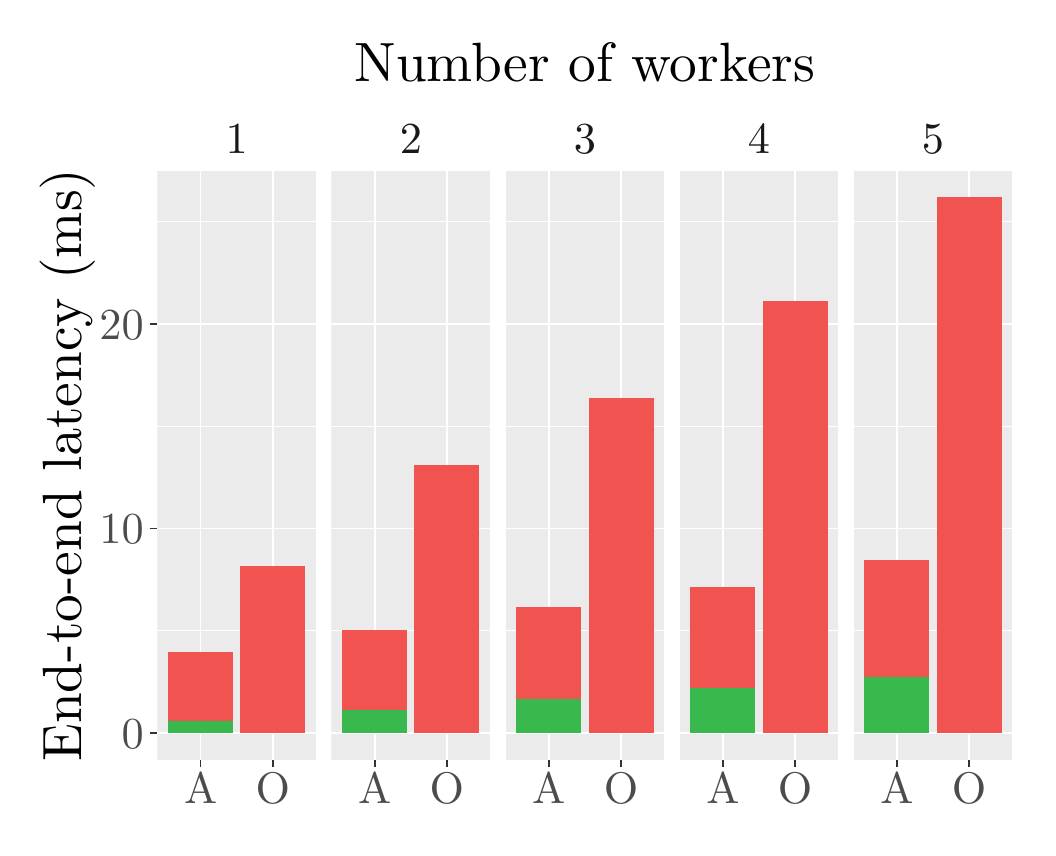
\begin{tikzpicture}[x=1pt,y=1pt]
\definecolor{fillColor}{RGB}{255,255,255}
\path[use as bounding box,fill=fillColor,fill opacity=0.00] (0,0) rectangle (361.35,289.08);
\begin{scope}
\path[clip] (  0.00,  0.00) rectangle (361.35,289.08);
\definecolor{drawColor}{RGB}{255,255,255}
\definecolor{fillColor}{RGB}{255,255,255}

\path[draw=drawColor,line width= 0.6pt,line join=round,line cap=round,fill=fillColor] (  0.00,  0.00) rectangle (361.35,289.08);
\end{scope}
\begin{scope}
\path[clip] ( 46.86, 24.58) rectangle (104.26,237.49);
\definecolor{fillColor}{gray}{0.92}

\path[fill=fillColor] ( 46.86, 24.58) rectangle (104.26,237.49);
\definecolor{drawColor}{RGB}{255,255,255}

\path[draw=drawColor,line width= 0.3pt,line join=round] ( 46.86, 71.18) --
	(104.26, 71.18);

\path[draw=drawColor,line width= 0.3pt,line join=round] ( 46.86,145.04) --
	(104.26,145.04);

\path[draw=drawColor,line width= 0.3pt,line join=round] ( 46.86,218.89) --
	(104.26,218.89);

\path[draw=drawColor,line width= 0.6pt,line join=round] ( 46.86, 34.26) --
	(104.26, 34.26);

\path[draw=drawColor,line width= 0.6pt,line join=round] ( 46.86,108.11) --
	(104.26,108.11);

\path[draw=drawColor,line width= 0.6pt,line join=round] ( 46.86,181.97) --
	(104.26,181.97);

\path[draw=drawColor,line width= 0.6pt,line join=round] ( 62.51, 24.58) --
	( 62.51,237.49);

\path[draw=drawColor,line width= 0.6pt,line join=round] ( 88.60, 24.58) --
	( 88.60,237.49);
\definecolor{fillColor}{RGB}{241,83,80}

\path[fill=fillColor] ( 76.86, 34.26) rectangle (100.34, 94.38);
\definecolor{fillColor}{RGB}{56,184,77}

\path[fill=fillColor] ( 50.77, 34.26) rectangle ( 74.25, 38.55);
\definecolor{fillColor}{RGB}{241,83,80}

\path[fill=fillColor] ( 50.77, 38.55) rectangle ( 74.25, 63.41);
\end{scope}
\begin{scope}
\path[clip] (109.76, 24.58) rectangle (167.16,237.49);
\definecolor{fillColor}{gray}{0.92}

\path[fill=fillColor] (109.76, 24.58) rectangle (167.16,237.49);
\definecolor{drawColor}{RGB}{255,255,255}

\path[draw=drawColor,line width= 0.3pt,line join=round] (109.76, 71.18) --
	(167.16, 71.18);

\path[draw=drawColor,line width= 0.3pt,line join=round] (109.76,145.04) --
	(167.16,145.04);

\path[draw=drawColor,line width= 0.3pt,line join=round] (109.76,218.89) --
	(167.16,218.89);

\path[draw=drawColor,line width= 0.6pt,line join=round] (109.76, 34.26) --
	(167.16, 34.26);

\path[draw=drawColor,line width= 0.6pt,line join=round] (109.76,108.11) --
	(167.16,108.11);

\path[draw=drawColor,line width= 0.6pt,line join=round] (109.76,181.97) --
	(167.16,181.97);

\path[draw=drawColor,line width= 0.6pt,line join=round] (125.41, 24.58) --
	(125.41,237.49);

\path[draw=drawColor,line width= 0.6pt,line join=round] (151.50, 24.58) --
	(151.50,237.49);
\definecolor{fillColor}{RGB}{241,83,80}

\path[fill=fillColor] (139.76, 34.26) rectangle (163.24,131.08);
\definecolor{fillColor}{RGB}{56,184,77}

\path[fill=fillColor] (113.67, 34.26) rectangle (137.15, 42.50);
\definecolor{fillColor}{RGB}{241,83,80}

\path[fill=fillColor] (113.67, 42.50) rectangle (137.15, 71.38);
\end{scope}
\begin{scope}
\path[clip] (172.66, 24.58) rectangle (230.05,237.49);
\definecolor{fillColor}{gray}{0.92}

\path[fill=fillColor] (172.66, 24.58) rectangle (230.05,237.49);
\definecolor{drawColor}{RGB}{255,255,255}

\path[draw=drawColor,line width= 0.3pt,line join=round] (172.66, 71.18) --
	(230.05, 71.18);

\path[draw=drawColor,line width= 0.3pt,line join=round] (172.66,145.04) --
	(230.05,145.04);

\path[draw=drawColor,line width= 0.3pt,line join=round] (172.66,218.89) --
	(230.05,218.89);

\path[draw=drawColor,line width= 0.6pt,line join=round] (172.66, 34.26) --
	(230.05, 34.26);

\path[draw=drawColor,line width= 0.6pt,line join=round] (172.66,108.11) --
	(230.05,108.11);

\path[draw=drawColor,line width= 0.6pt,line join=round] (172.66,181.97) --
	(230.05,181.97);

\path[draw=drawColor,line width= 0.6pt,line join=round] (188.31, 24.58) --
	(188.31,237.49);

\path[draw=drawColor,line width= 0.6pt,line join=round] (214.40, 24.58) --
	(214.40,237.49);
\definecolor{fillColor}{RGB}{241,83,80}

\path[fill=fillColor] (202.66, 34.26) rectangle (226.14,155.30);
\definecolor{fillColor}{RGB}{56,184,77}

\path[fill=fillColor] (176.57, 34.26) rectangle (200.05, 46.46);
\definecolor{fillColor}{RGB}{241,83,80}

\path[fill=fillColor] (176.57, 46.46) rectangle (200.05, 79.65);
\end{scope}
\begin{scope}
\path[clip] (235.55, 24.58) rectangle (292.95,237.49);
\definecolor{fillColor}{gray}{0.92}

\path[fill=fillColor] (235.55, 24.58) rectangle (292.95,237.49);
\definecolor{drawColor}{RGB}{255,255,255}

\path[draw=drawColor,line width= 0.3pt,line join=round] (235.55, 71.18) --
	(292.95, 71.18);

\path[draw=drawColor,line width= 0.3pt,line join=round] (235.55,145.04) --
	(292.95,145.04);

\path[draw=drawColor,line width= 0.3pt,line join=round] (235.55,218.89) --
	(292.95,218.89);

\path[draw=drawColor,line width= 0.6pt,line join=round] (235.55, 34.26) --
	(292.95, 34.26);

\path[draw=drawColor,line width= 0.6pt,line join=round] (235.55,108.11) --
	(292.95,108.11);

\path[draw=drawColor,line width= 0.6pt,line join=round] (235.55,181.97) --
	(292.95,181.97);

\path[draw=drawColor,line width= 0.6pt,line join=round] (251.21, 24.58) --
	(251.21,237.49);

\path[draw=drawColor,line width= 0.6pt,line join=round] (277.30, 24.58) --
	(277.30,237.49);
\definecolor{fillColor}{RGB}{241,83,80}

\path[fill=fillColor] (265.56, 34.26) rectangle (289.04,190.48);
\definecolor{fillColor}{RGB}{56,184,77}

\path[fill=fillColor] (239.47, 34.26) rectangle (262.95, 50.61);
\definecolor{fillColor}{RGB}{241,83,80}

\path[fill=fillColor] (239.47, 50.61) rectangle (262.95, 86.88);
\end{scope}
\begin{scope}
\path[clip] (298.45, 24.58) rectangle (355.85,237.49);
\definecolor{fillColor}{gray}{0.92}

\path[fill=fillColor] (298.45, 24.58) rectangle (355.85,237.49);
\definecolor{drawColor}{RGB}{255,255,255}

\path[draw=drawColor,line width= 0.3pt,line join=round] (298.45, 71.18) --
	(355.85, 71.18);

\path[draw=drawColor,line width= 0.3pt,line join=round] (298.45,145.04) --
	(355.85,145.04);

\path[draw=drawColor,line width= 0.3pt,line join=round] (298.45,218.89) --
	(355.85,218.89);

\path[draw=drawColor,line width= 0.6pt,line join=round] (298.45, 34.26) --
	(355.85, 34.26);

\path[draw=drawColor,line width= 0.6pt,line join=round] (298.45,108.11) --
	(355.85,108.11);

\path[draw=drawColor,line width= 0.6pt,line join=round] (298.45,181.97) --
	(355.85,181.97);

\path[draw=drawColor,line width= 0.6pt,line join=round] (314.11, 24.58) --
	(314.11,237.49);

\path[draw=drawColor,line width= 0.6pt,line join=round] (340.20, 24.58) --
	(340.20,237.49);
\definecolor{fillColor}{RGB}{241,83,80}

\path[fill=fillColor] (328.46, 34.26) rectangle (351.94,227.81);
\definecolor{fillColor}{RGB}{56,184,77}

\path[fill=fillColor] (302.37, 34.26) rectangle (325.85, 54.27);
\definecolor{fillColor}{RGB}{241,83,80}

\path[fill=fillColor] (302.37, 54.27) rectangle (325.85, 96.66);
\end{scope}
\begin{scope}
\path[clip] ( 46.86,237.49) rectangle (104.26,260.42);
\definecolor{drawColor}{RGB}{255,255,255}

\path[draw=drawColor,line width= 0.6pt,line join=round,line cap=round] ( 46.86,237.49) rectangle (104.26,260.42);
\definecolor{drawColor}{gray}{0.10}

\node[text=drawColor,anchor=base,inner sep=0pt, outer sep=0pt, scale=  1.60] at ( 75.56,243.44) {1};
\end{scope}
\begin{scope}
\path[clip] (109.76,237.49) rectangle (167.16,260.42);
\definecolor{drawColor}{RGB}{255,255,255}

\path[draw=drawColor,line width= 0.6pt,line join=round,line cap=round] (109.76,237.49) rectangle (167.16,260.42);
\definecolor{drawColor}{gray}{0.10}

\node[text=drawColor,anchor=base,inner sep=0pt, outer sep=0pt, scale=  1.60] at (138.46,243.44) {2};
\end{scope}
\begin{scope}
\path[clip] (172.66,237.49) rectangle (230.05,260.42);
\definecolor{drawColor}{RGB}{255,255,255}

\path[draw=drawColor,line width= 0.6pt,line join=round,line cap=round] (172.66,237.49) rectangle (230.05,260.42);
\definecolor{drawColor}{gray}{0.10}

\node[text=drawColor,anchor=base,inner sep=0pt, outer sep=0pt, scale=  1.60] at (201.35,243.44) {3};
\end{scope}
\begin{scope}
\path[clip] (235.55,237.49) rectangle (292.95,260.42);
\definecolor{drawColor}{RGB}{255,255,255}

\path[draw=drawColor,line width= 0.6pt,line join=round,line cap=round] (235.55,237.49) rectangle (292.95,260.42);
\definecolor{drawColor}{gray}{0.10}

\node[text=drawColor,anchor=base,inner sep=0pt, outer sep=0pt, scale=  1.60] at (264.25,243.44) {4};
\end{scope}
\begin{scope}
\path[clip] (298.45,237.49) rectangle (355.85,260.42);
\definecolor{drawColor}{RGB}{255,255,255}

\path[draw=drawColor,line width= 0.6pt,line join=round,line cap=round] (298.45,237.49) rectangle (355.85,260.42);
\definecolor{drawColor}{gray}{0.10}

\node[text=drawColor,anchor=base,inner sep=0pt, outer sep=0pt, scale=  1.60] at (327.15,243.44) {5};
\end{scope}
\begin{scope}
\path[clip] (  0.00,  0.00) rectangle (361.35,289.08);
\definecolor{drawColor}{gray}{0.20}

\path[draw=drawColor,line width= 0.6pt,line join=round] ( 62.51, 21.83) --
	( 62.51, 24.58);

\path[draw=drawColor,line width= 0.6pt,line join=round] ( 88.60, 21.83) --
	( 88.60, 24.58);
\end{scope}
\begin{scope}
\path[clip] (  0.00,  0.00) rectangle (361.35,289.08);
\definecolor{drawColor}{gray}{0.30}

\node[text=drawColor,anchor=base,inner sep=0pt, outer sep=0pt, scale=  1.60] at ( 62.51,  8.61) {A};

\node[text=drawColor,anchor=base,inner sep=0pt, outer sep=0pt, scale=  1.60] at ( 88.60,  8.61) {O};
\end{scope}
\begin{scope}
\path[clip] (  0.00,  0.00) rectangle (361.35,289.08);
\definecolor{drawColor}{gray}{0.20}

\path[draw=drawColor,line width= 0.6pt,line join=round] (125.41, 21.83) --
	(125.41, 24.58);

\path[draw=drawColor,line width= 0.6pt,line join=round] (151.50, 21.83) --
	(151.50, 24.58);
\end{scope}
\begin{scope}
\path[clip] (  0.00,  0.00) rectangle (361.35,289.08);
\definecolor{drawColor}{gray}{0.30}

\node[text=drawColor,anchor=base,inner sep=0pt, outer sep=0pt, scale=  1.60] at (125.41,  8.61) {A};

\node[text=drawColor,anchor=base,inner sep=0pt, outer sep=0pt, scale=  1.60] at (151.50,  8.61) {O};
\end{scope}
\begin{scope}
\path[clip] (  0.00,  0.00) rectangle (361.35,289.08);
\definecolor{drawColor}{gray}{0.20}

\path[draw=drawColor,line width= 0.6pt,line join=round] (188.31, 21.83) --
	(188.31, 24.58);

\path[draw=drawColor,line width= 0.6pt,line join=round] (214.40, 21.83) --
	(214.40, 24.58);
\end{scope}
\begin{scope}
\path[clip] (  0.00,  0.00) rectangle (361.35,289.08);
\definecolor{drawColor}{gray}{0.30}

\node[text=drawColor,anchor=base,inner sep=0pt, outer sep=0pt, scale=  1.60] at (188.31,  8.61) {A};

\node[text=drawColor,anchor=base,inner sep=0pt, outer sep=0pt, scale=  1.60] at (214.40,  8.61) {O};
\end{scope}
\begin{scope}
\path[clip] (  0.00,  0.00) rectangle (361.35,289.08);
\definecolor{drawColor}{gray}{0.20}

\path[draw=drawColor,line width= 0.6pt,line join=round] (251.21, 21.83) --
	(251.21, 24.58);

\path[draw=drawColor,line width= 0.6pt,line join=round] (277.30, 21.83) --
	(277.30, 24.58);
\end{scope}
\begin{scope}
\path[clip] (  0.00,  0.00) rectangle (361.35,289.08);
\definecolor{drawColor}{gray}{0.30}

\node[text=drawColor,anchor=base,inner sep=0pt, outer sep=0pt, scale=  1.60] at (251.21,  8.61) {A};

\node[text=drawColor,anchor=base,inner sep=0pt, outer sep=0pt, scale=  1.60] at (277.30,  8.61) {O};
\end{scope}
\begin{scope}
\path[clip] (  0.00,  0.00) rectangle (361.35,289.08);
\definecolor{drawColor}{gray}{0.20}

\path[draw=drawColor,line width= 0.6pt,line join=round] (314.11, 21.83) --
	(314.11, 24.58);

\path[draw=drawColor,line width= 0.6pt,line join=round] (340.20, 21.83) --
	(340.20, 24.58);
\end{scope}
\begin{scope}
\path[clip] (  0.00,  0.00) rectangle (361.35,289.08);
\definecolor{drawColor}{gray}{0.30}

\node[text=drawColor,anchor=base,inner sep=0pt, outer sep=0pt, scale=  1.60] at (314.11,  8.61) {A};

\node[text=drawColor,anchor=base,inner sep=0pt, outer sep=0pt, scale=  1.60] at (340.20,  8.61) {O};
\end{scope}
\begin{scope}
\path[clip] (  0.00,  0.00) rectangle (361.35,289.08);
\definecolor{drawColor}{gray}{0.30}

\node[text=drawColor,anchor=base east,inner sep=0pt, outer sep=0pt, scale=  1.60] at ( 41.91, 28.75) {0};

\node[text=drawColor,anchor=base east,inner sep=0pt, outer sep=0pt, scale=  1.60] at ( 41.91,102.60) {10};

\node[text=drawColor,anchor=base east,inner sep=0pt, outer sep=0pt, scale=  1.60] at ( 41.91,176.46) {20};
\end{scope}
\begin{scope}
\path[clip] (  0.00,  0.00) rectangle (361.35,289.08);
\definecolor{drawColor}{gray}{0.20}

\path[draw=drawColor,line width= 0.6pt,line join=round] ( 44.11, 34.26) --
	( 46.86, 34.26);

\path[draw=drawColor,line width= 0.6pt,line join=round] ( 44.11,108.11) --
	( 46.86,108.11);

\path[draw=drawColor,line width= 0.6pt,line join=round] ( 44.11,181.97) --
	( 46.86,181.97);
\end{scope}
\begin{scope}
\path[clip] (  0.00,  0.00) rectangle (361.35,289.08);
\definecolor{drawColor}{RGB}{0,0,0}

\node[text=drawColor,rotate= 90.00,anchor=base,inner sep=0pt, outer sep=0pt, scale=  2.00] at ( 19.27,131.03) {End-to-end latency (ms)};
\end{scope}
\begin{scope}
\path[clip] (  0.00,  0.00) rectangle (361.35,289.08);
\definecolor{drawColor}{RGB}{0,0,0}

\node[text=drawColor,anchor=base,inner sep=0pt, outer sep=0pt, scale=  2.00] at (201.35,269.81) {Number of workers};
\end{scope}
\end{tikzpicture}
